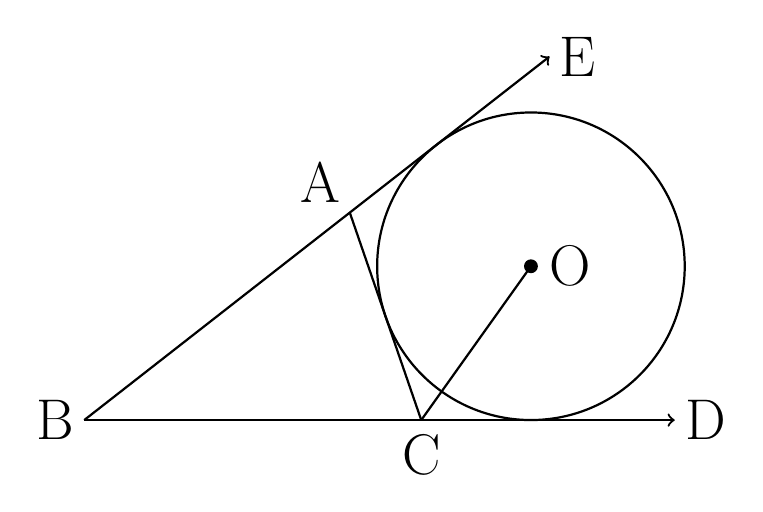
\begin{tikzpicture}[scale=1]

    % --- Geometric Constants ---
    % Angle of the main vertex B is 38 degrees
    % Center O lies on the angle bisector (19 degrees)
    % Distance BO = 6, Radius = 6 * sin(19) approx 1.953
    % For tangency at AC, distance BM = BO - radius = 4.047
    % Side lengths BA = BC = BM / cos(19) approx 4.28

    % --- Coordinates ---
    \coordinate (B) at (0,0);
    \coordinate (O) at (19:6);
    \coordinate (A) at (38:4.28);
    \coordinate (C) at (4.28,0);
    
    % Ray endpoints for labels E and D
    \coordinate (E_end) at (38:7.5);
    \coordinate (D_end) at (0:7.5);

    % --- Drawing Elements ---
    
    % Rays BE and BD with arrows
    \draw[thick, ->] (B) -- (E_end) node[right, font=\huge] {E};
    \draw[thick, ->] (B) -- (D_end) node[right, font=\huge] {D};
    
    % Triangle segment AC (Correctly tangent to the circle)
    \draw[thick] (A) -- (C);
    
    % The Excircle
    \draw[thick] (O) circle (1.953);
    
    % Center point O and connecting segment OC
    \fill (O) circle (2.5pt);
    \draw[thick] (O) -- (C);

    % --- Point Labels (Extra Large) ---
    % Positioned exactly as shown in Figure 14
    \node[left, font=\huge] at (B) {B};
    \node[above left, font=\huge] at (A) {A};
    \node[below, font=\huge, yshift=-2pt] at (C) {C};
    \node[right, font=\huge, xshift=3pt] at (O) {O};

\end{tikzpicture}